\chapter{Implementasi dan Pengujian}
\label{chap:implementasipengujian}
Pada bab ini akan diimplementasikan kode program untuk propagasi email dan pengujian dua skenario yang ada pada Bab ~\ref{chap:hasilstudi}.

\section{Lingkungan Implementasi}
\label{sec:lingkunganimplementasi}
Implementasi dilakukan pada lingkungan :
\begin{enumerate}
	\item Eclipse 4.5 Mars
	\item BPMN versi 2.0 dan Camunda Modeler versi 1.7.2.
	\item BPMS Camunda versi 7.6.0 dan berjalan pada tomcat versi 8.0.24.
	
\end{enumerate}

\section{Implementasi Algoritma Pengiriman Email}
\label{implementasialgo}
Beberapa potongan kode di bawah ini adalah kode untuk pengiriman email. Kode secara keseluruhan dapat dilihat pada Lampiran~\ref{lamp:tasklistener}
\begin{itemize}
	\item Konfigurasi email admin.
\begin{lstlisting}[language=Java,basicstyle=\tiny,caption=TaskAssignmentListener.java]
  private static final String HOST = "smtp.gmail.com";
  private static final String USER = "camundasys@gmail.com";
  private static final String PWD = "epW3S4KN";
\end{lstlisting}
	

	\item Kode untuk mengambil assignee (aktor dari \textit{task}, mengambil id \textit{task}, dan mengambil alamat email aktor. Method notify() dipanggil ketika \textit{event listener} pada\textit{task} dipanggil. Misalnya suatu \textit{task} yang menggunakan \textit{event listener create} akan memanggil method notify() ketika \textit{task} dibuat.
	\begin{lstlisting}[language=Java,basicstyle=\tiny,caption=TaskAssignmentListener.java]

 public void notify(DelegateTask delegateTask) {
    String assignee = delegateTask.getAssignee();
    String taskId = delegateTask.getId();
\end{lstlisting}

	\item Konfigurasi SMTP Gmail.
	\begin{lstlisting}[language=Java,basicstyle=\tiny,caption=TaskAssignmentListener.java]

               props = System.getProperties();
               props.put("mail.smtp.port", "587");
               props.put("mail.smtp.auth", "true");
               props.put("mail.smtp.starttls.enable", "true");

\end{lstlisting}
	\item Kode untuk mendapatkan aktor apabila atribut assignee pada BPMN memiliki nilai.
	\begin{lstlisting}[language=Java,basicstyle=\tiny,caption =TaskAssignmentListener.java]
	if (assignee != null) {
      IdentityService identityService = Context.getProcessEngineConfiguration().getIdentityService();
      User user = identityService.createUserQuery().userId(assignee).singleResult();
      if (user != null) {
    	  this.sendEmail(user);
      }
    }
	\end{lstlisting}
	
		\item Kode untuk mendapatkan aktor apabila atribut assignee pada BPMN tidak memiliki nilai. Kode ini mengambil aktor yang pada \textit{Candidate User} atau \textit{Candidate Group}.
	\begin{lstlisting}[language=Java,basicstyle=\tiny,caption =TaskAssignmentListener.java]
	    	TaskEntity task = (TaskEntity)delegateTask;
    	List<IdentityLinkEntity> identityLinks = task.getIdentityLinks();
    	
    	for(IdentityLinkEntity link : identityLinks) {
    		if(link.getType().equals(IdentityLinkType.CANDIDATE)) {
    		    if(link.isUser()) {
	    		     User user = Context.getProcessEngineConfiguration().getIdentityService().createUserQuery().userId(link.getUserId()).singleResult();
	    		     sendEmail(user);
    		    }
    		    if(link.isGroup()) {
    		        List<User> users = Context.getProcessEngineConfiguration().getIdentityService().createUserQuery().memberOfGroup(link.getGroupId()).list();
    		        for(User user : users) {
    		        	sendEmail(user);
    		        }
    		    }
    		}
    	}
	\end{lstlisting}
	
	

	\item Kode untuk membangkitkan subjek dan isi email. Kelas Properties menyimpan konfigurasi email yang akan digunakan. 
	\begin{lstlisting}[language=Java,basicstyle=\tiny,caption=TaskAssignmentListener.java]
 props = System.getProperties();
          props.put("mail.smtp.port", "587");
          props.put("mail.smtp.auth", "true");
          props.put("mail.smtp.starttls.enable", "true");
					
 session = Session.getDefaultInstance(props, null);
               message = new MimeMessage(session);
               message.addRecipient(Message.RecipientType.TO, new InternetAddress(recipient));
               message.setSubject("Task " + delegateTask.getName());
               
String name = user.getFirstName();
          String emailBody ="";
          emailBody += "Dear "+name+",<br>";
          emailBody += "Anda mendapatkan task " +taskName + " untuk dikerjakan.<br>";
          emailBody += "Segera akses http://localhost:1234/camunda/app/tasklist/default/#/?task="+taskId +" untuk menjalankannya.<br>";
          emailBody += "Terima kasih.";
          message.setContent(emailBody, "text/html");

\end{lstlisting}

	\item Kode untuk mengirimkan email.
	\begin{lstlisting}[language=Java,basicstyle=\tiny,caption=TaskAssignmentListener.java]

Transport transport = session.getTransport("smtp");            
               transport.connect(HOST, USER, PWD);
               transport.sendMessage(message, message.getAllRecipients());
               transport.close();
\end{lstlisting}
	
\end{itemize}
Implementasi algoritma pengiriman email (TaskAssignmentListener.java) dikaitkan dengan setiap \textit{user task} pada BPMN menggunakan \textit{event create}. Contohnya adalah sebagai berikut :
	\begin{figure}[H]
			\centering
			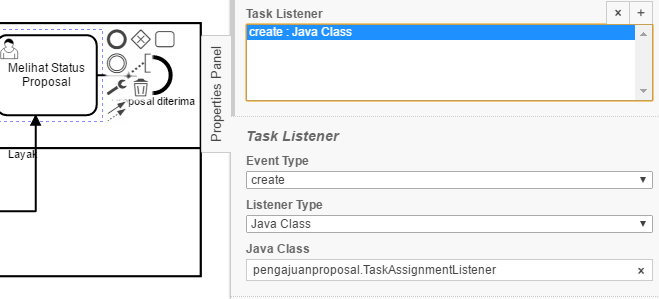
\includegraphics[scale=0.8]{Gambar/Bab-5/taskListener}
			\caption{Task Listener pada BPMN} 
			\label{fig:pengujian_taskListener}
	\end{figure}




\section{Pengujian}
\label{sec:pengujian}
Pengujian dilakukan pada skenario yang ada pada subbab \ref{hasilstudi_bpmn_masalah} Masalah Proses Bisnis. Ada dua skenario yang diuji, yaitu Pengajuan Proposal dan Pendaftaran BPJS. Kriteria yang diuji adalah berhasil atau tidaknya pengiriman email ke masing-masing aktor dan waktu yang diperlukan untuk mengirim email. Pengujian melibatkan tiga aktor, yaitu : 
\begin{enumerate}
	\item John, dengan alamat email johncamunda@gmail.com dan bagian dari grup \textit{sales}.
	\item Mary, dengan alamat email marycamunda@yahoo.com dan bagian dari grup \textit{accounting}.
	\item Peter, dengan alamat email petercamunda@gmail.com dan bagian dari grup \textit{management}.
\end{enumerate}



\subsection{Hasil Pengujian Kasus Pengajuan Proposal}
\label{pengujian_kasus1}
Workflow Pengajuan Proposal dapat dilihat pada subbab \ref{hasilstudi_workflow}
\begin{enumerate}
	\item Memulai proses Pengajuan Proposal pada 2:18 PM
		\begin{figure}[H]
			\centering
			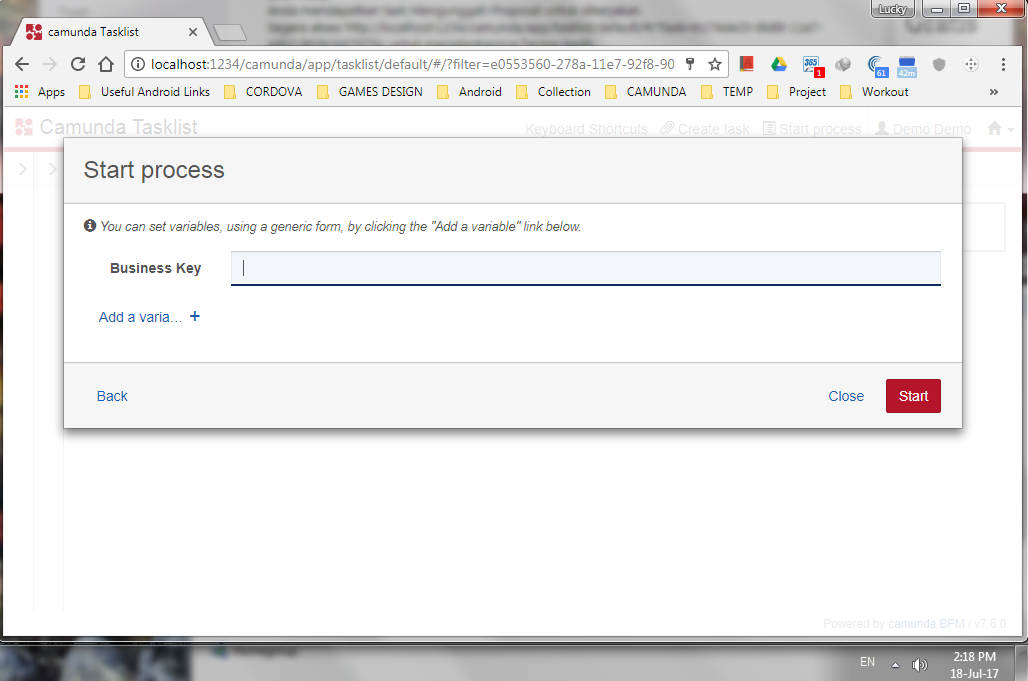
\includegraphics[scale=0.5]{Gambar/Bab-5/kasus1/1}
			\caption{Memulai Proses Pengajuan Proposal} 
			\label{fig:pengujian_kasus1_1}
	\end{figure}
	
		\item John dan Mary menerima email untuk mengunggah proposal pada 2:18 PM
		\begin{figure}[H]
			\centering
			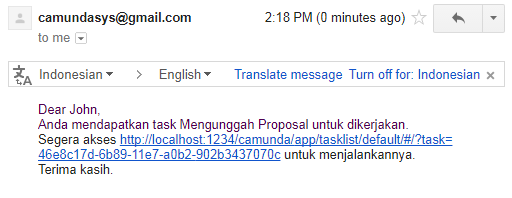
\includegraphics[scale=0.8]{Gambar/Bab-5/kasus1/2}
			\caption{Email Mengunggah Proposal} 
			\label{fig:pengujian_kasus1_2}
	\end{figure}
	
		\begin{figure}[H]
			\centering
			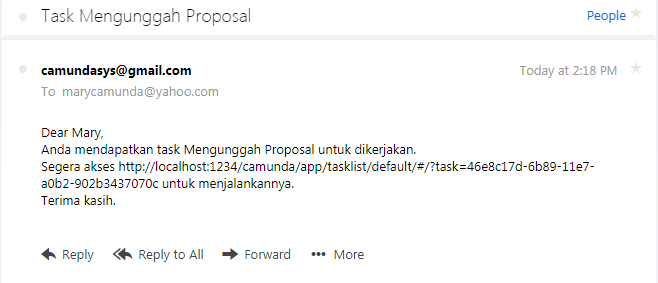
\includegraphics[scale=0.8]{Gambar/Bab-5/kasus1/3}
			\caption{Email Mengunggah Proposal} 
			\label{fig:pengujian_kasus1_3}
	\end{figure}
	
		\item John mengklaim \textit{task} dan mengunggah proposal pada 2:21 PM 
		\begin{figure}[H]
			\centering
			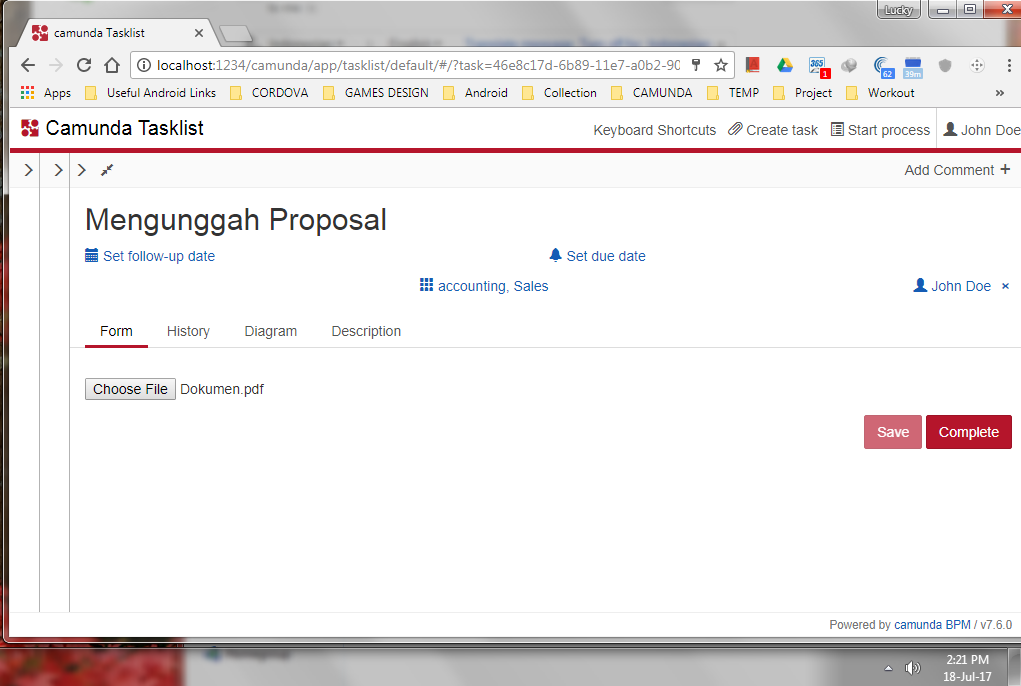
\includegraphics[scale=0.5]{Gambar/Bab-5/kasus1/4}
			\caption{Mengunggah Proposal} 
			\label{fig:pengujian_kasus1_4}
	\end{figure}
	
		\item Peter menerima email untuk memeriksa proposal pada 2:21 PM
		\begin{figure}[H]
			\centering
			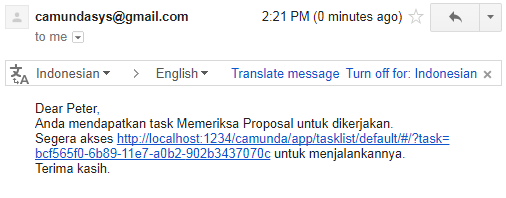
\includegraphics[scale=0.8]{Gambar/Bab-5/kasus1/5}
			\caption{Email Memeriksa Proposal} 
			\label{fig:pengujian_kasus1_5}
	\end{figure}
	
		\item Peter memeriksa proposal pada 2:23 PM
		\begin{figure}[H]
			\centering
			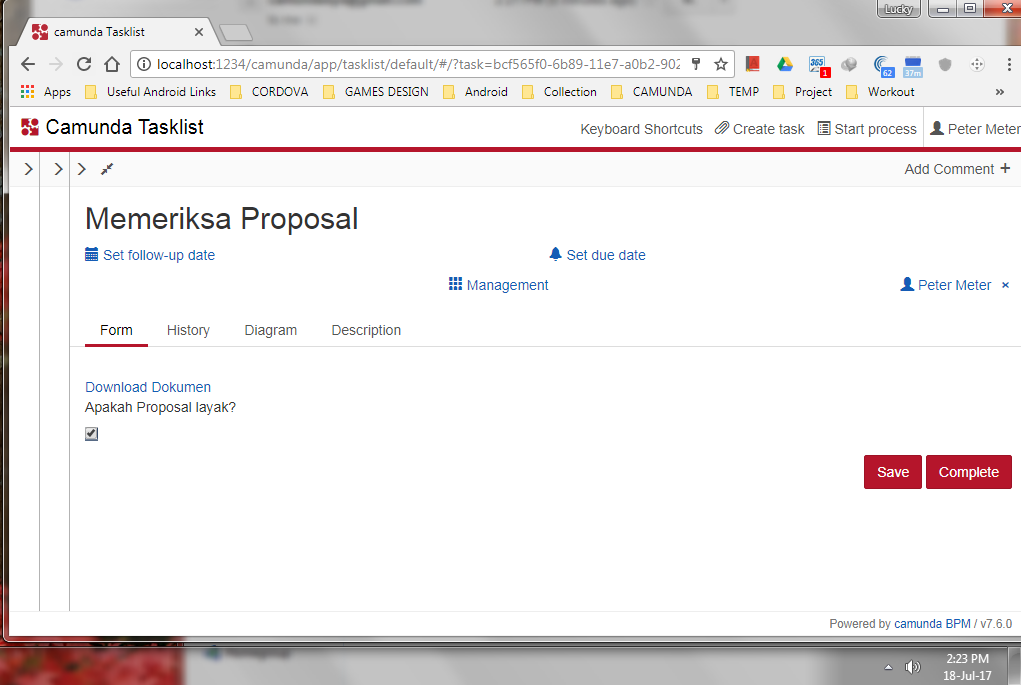
\includegraphics[scale=0.5]{Gambar/Bab-5/kasus1/6}
			\caption{Peter Memeriksa Proposal} 
			\label{fig:pengujian_kasus1_6}
	\end{figure}
	
		\item John menerima email untuk melihat status proposal pada 2:23 PM
		\begin{figure}[H]
			\centering
			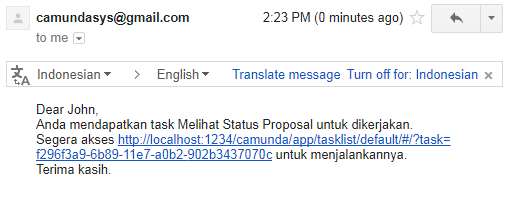
\includegraphics[scale=0.8]{Gambar/Bab-5/kasus1/7}
			\caption{Email Melihat Status Proposal} 
			\label{fig:pengujian_kasus1_7}
	\end{figure}
	
		\item John melihat status proposal pada 2:24 PM
		\begin{figure}[H]
			\centering
			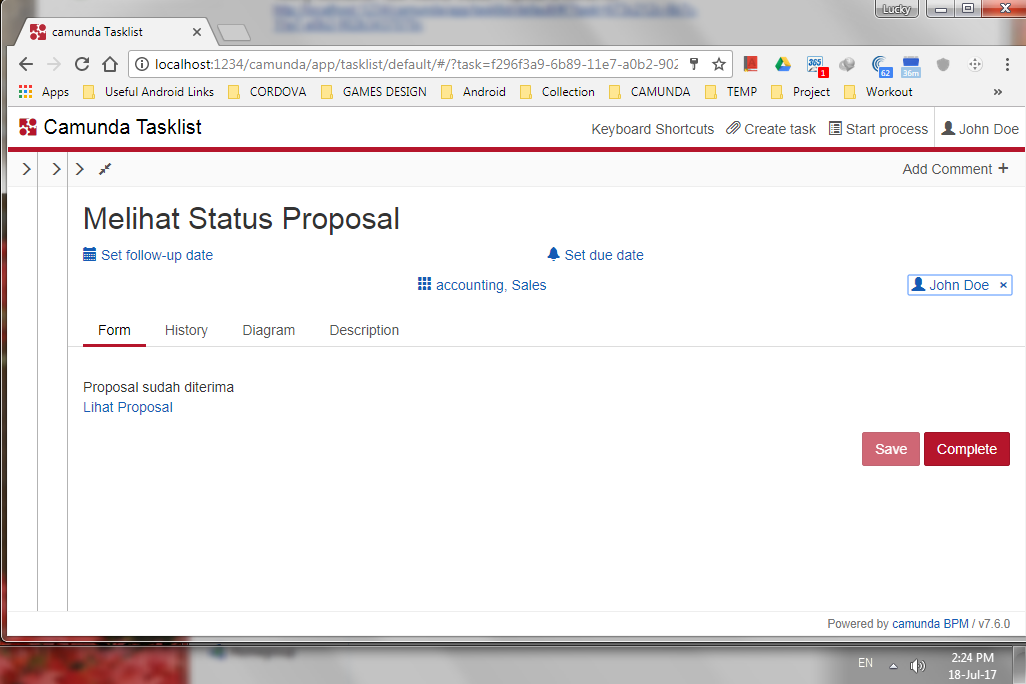
\includegraphics[scale=0.5]{Gambar/Bab-5/kasus1/8}
			\caption{John Melihat Status Proposal} 
			\label{fig:pengujian_kasus1_8}
	\end{figure}


\end{enumerate}



\subsection{Hasil Pengujian Kasus Pendaftaran BPJS}
\label{pengujian_kasus2}
Workflow Kasus Pendaftaran BPJS dapat dilihat pada subbab \ref{hasilstudi_workflow}
\begin{enumerate}
	\item Proses Pendaftaran BPJS dimulai pukul 2:40 PM.
			\begin{figure}[H]
			\centering
			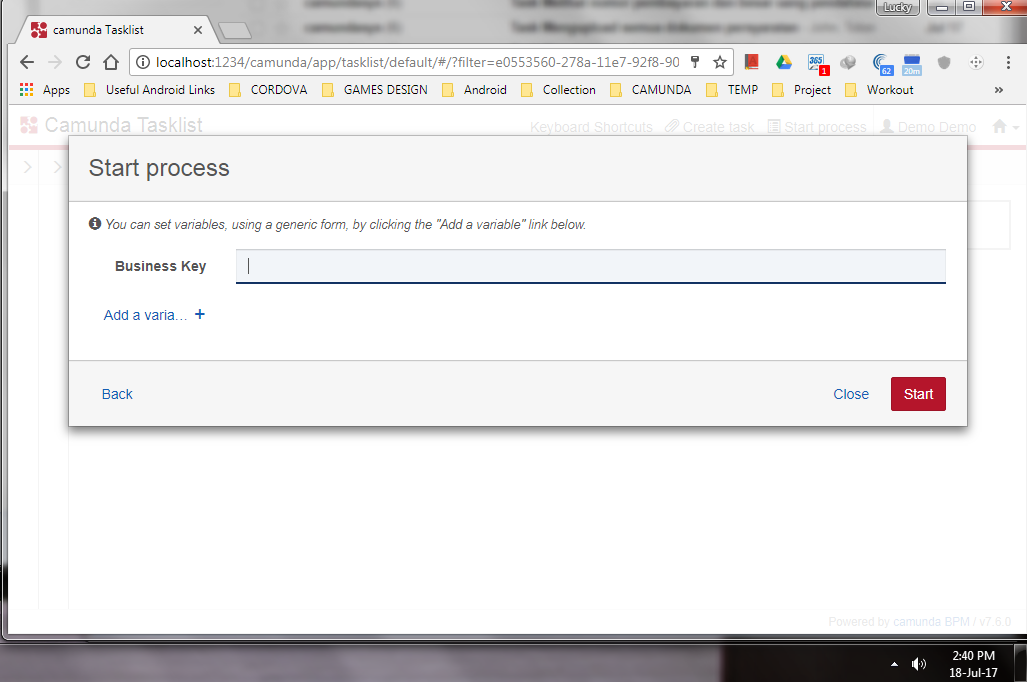
\includegraphics[scale=0.5]{Gambar/Bab-5/kasus2/1}
			\caption{Memulai Proses Pendaftaran BPJS} 
			\label{fig:pengujian_kasus2_1}
	\end{figure}
	

	\item John menerima email untuk mengisi formulir pendaftaran BPJS pada pukul 2:40PM.
			\begin{figure}[H]
			\centering
			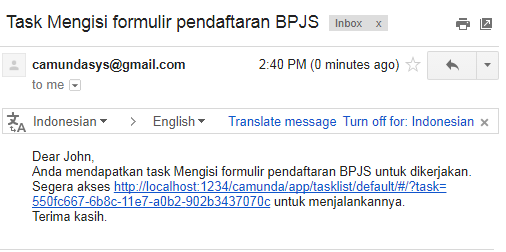
\includegraphics[scale=0.8]{Gambar/Bab-5/kasus2/2}
			\caption{Email Mengisi Formulir Pendaftaran BPJS} 
			\label{fig:pengujian_kasus2_2}
	\end{figure}
	

	\item John mengisi formulir pendaftaran BPJS pukul 2:41 PM
			\begin{figure}[H]
			\centering
			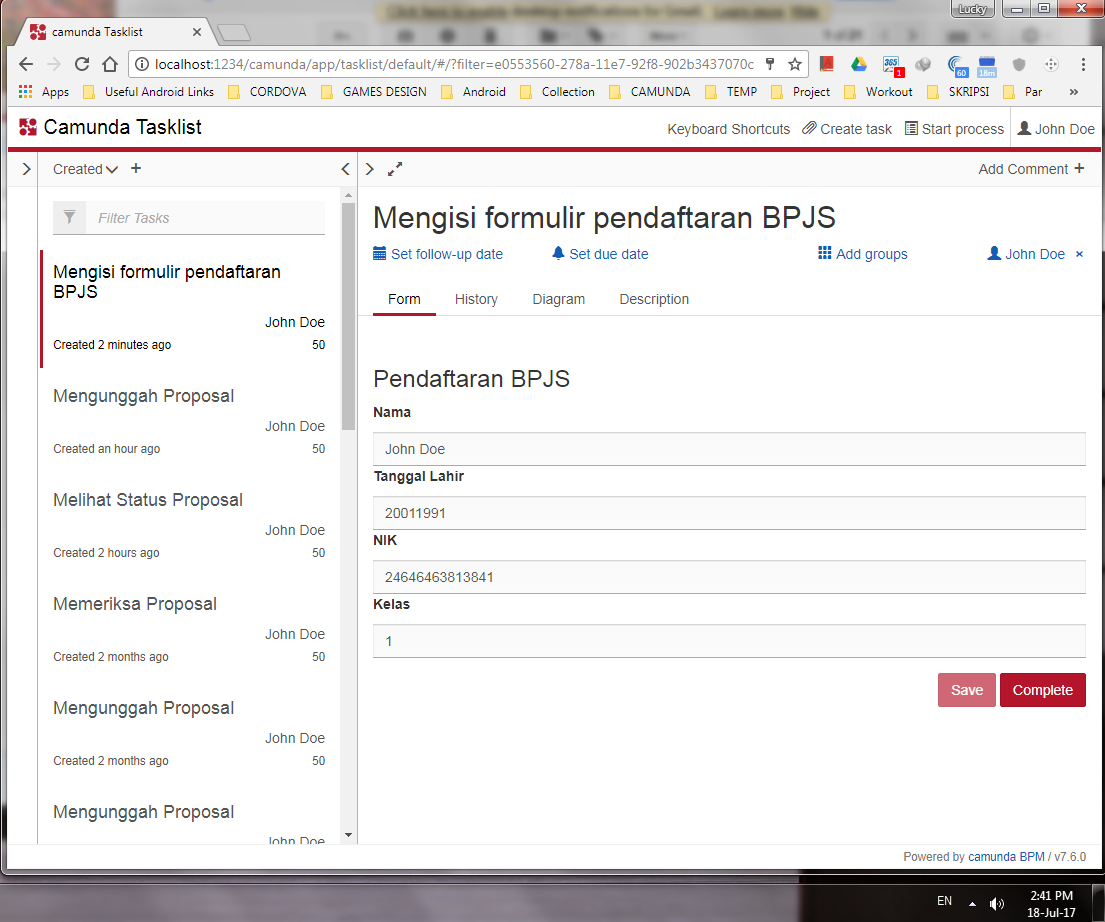
\includegraphics[scale=0.5]{Gambar/Bab-5/kasus2/3}
			\caption{Mengisi Formulir Pendaftaran BPJS} 
			\label{fig:pengujian_kasus2_3}
	\end{figure}
	

	\item John menerima email untuk mengunggah semua dokumen persyaratan pada pukul 2:42 PM.
			\begin{figure}[H]
			\centering 
			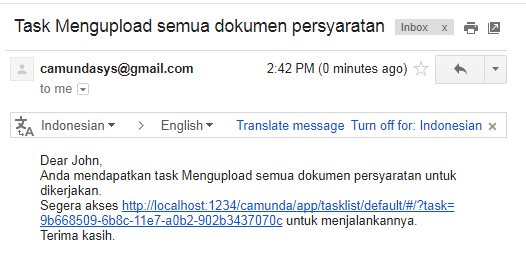
\includegraphics[scale=0.8]{Gambar/Bab-5/kasus2/4}
			\caption{Email Mengunggah Dokumen Persyaratan} 
			\label{fig:pengujian_kasus2_4}
	\end{figure}
	

	\item John mengunggah semua dokumen persyaratan pada pukul 2:43 PM
			\begin{figure}[H]
			\centering
			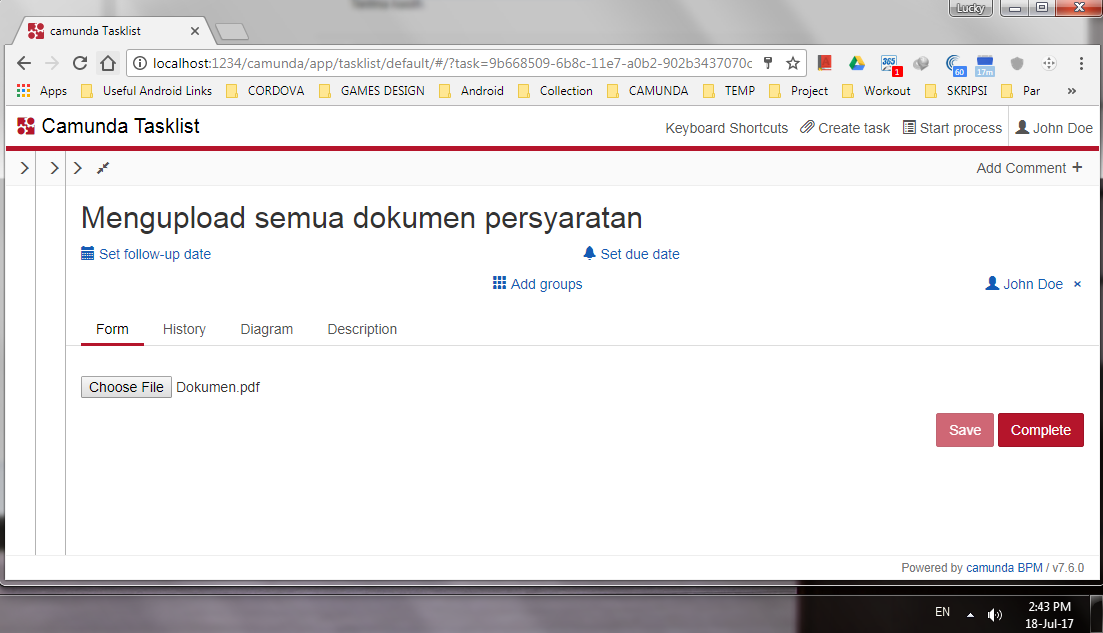
\includegraphics[scale=0.5]{Gambar/Bab-5/kasus2/5}
			\caption{Mengunggah Dokumen Persyaratan} 
			\label{fig:pengujian_kasus2_5}
	\end{figure}
	

	\item John menerima email untuk melihat nomor pembayaran dan besar uang pendaftaran pada pukul 2:43 PM
			\begin{figure}[H]
			\centering
			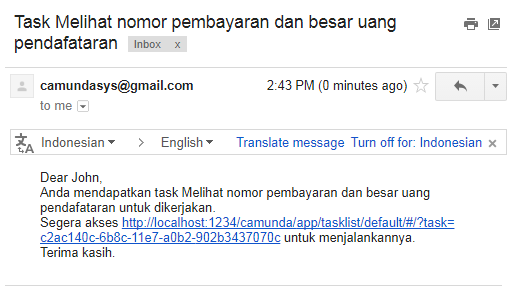
\includegraphics[scale=0.8]{Gambar/Bab-5/kasus2/6}
			\caption{Email Nomor Pembayaran dan Uang Pendaftaran} 
			\label{fig:pengujian_kasus2_6}
	\end{figure}
	

	\item John melihat nomor pembayaran dan besar uang pendaftaran pada pukul 2:44 PM
			\begin{figure}[H]
			\centering
			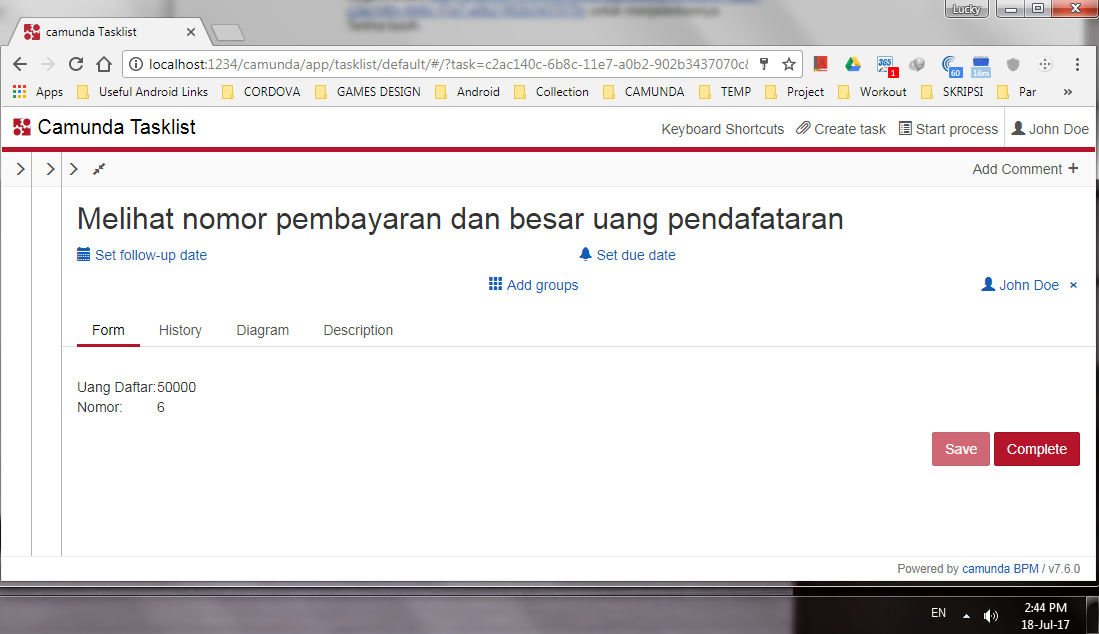
\includegraphics[scale=0.5]{Gambar/Bab-5/kasus2/7}
			\caption{Melihat Nomor Pembayaran dan Uang Pendaftaran} 
			\label{fig:pengujian_kasus2_7}
	\end{figure}
	

	\item John menerima email untuk memilih jadwal verifikasi dokumen pada pukul 2:43 PM
			\begin{figure}[H]
			\centering
			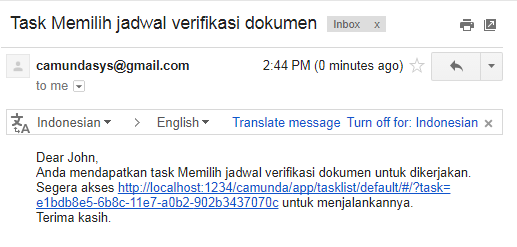
\includegraphics[scale=0.8]{Gambar/Bab-5/kasus2/8}
			\caption{Email Memilih Jadwal Verifikasi Dokumen} 
			\label{fig:pengujian_kasus2_8}
	\end{figure}
	

	\item John memilih jadwal verifikasi dokumen pada pukul 2:44 PM
			\begin{figure}[H]
			\centering
			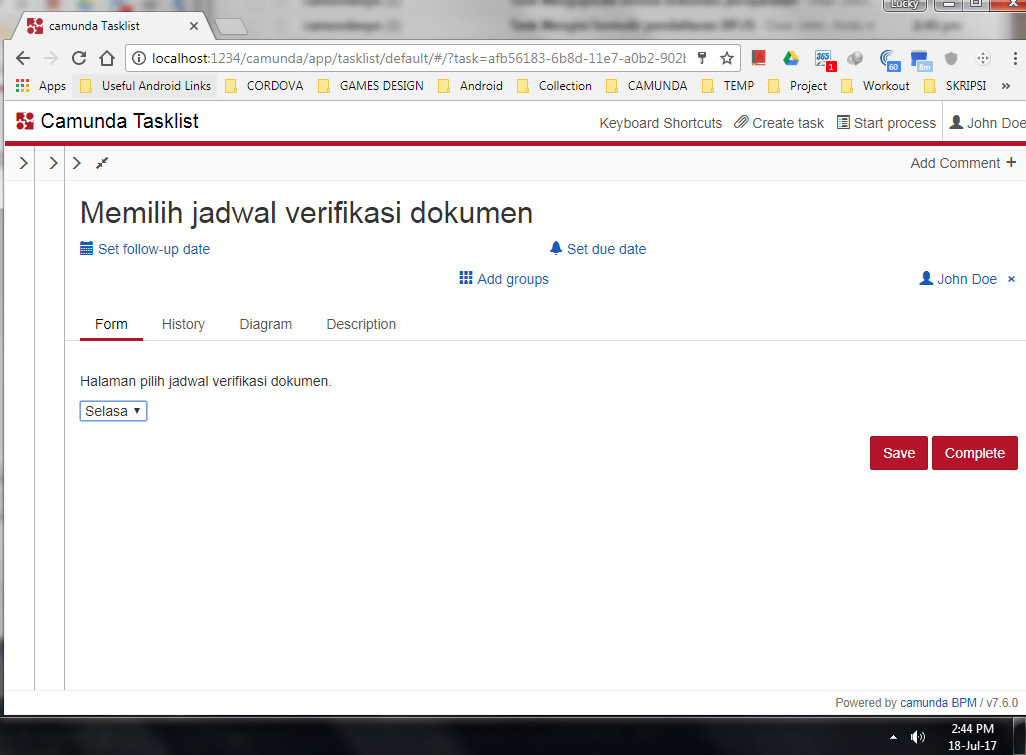
\includegraphics[scale=0.5]{Gambar/Bab-5/kasus2/9}
			\caption{Memilih Jadwal Verifikasi Dokumen} 
			\label{fig:pengujian_kasus2_9}
	\end{figure}
	

	\item John menerima email untuk mencetak jadwal dan nomor antrian pada pukul 2:44 PM
			\begin{figure}[H]
			\centering
			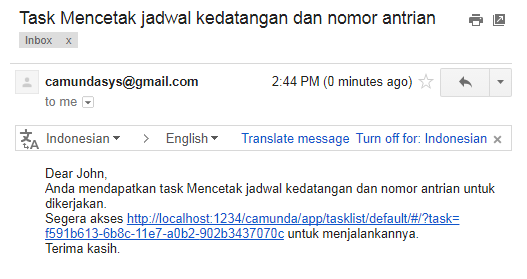
\includegraphics[scale=0.8]{Gambar/Bab-5/kasus2/10}
			\caption{Email Mencetak Jadwal} 
			\label{fig:pengujian_kasus2_10}
	\end{figure}
	

	\item John mencetak jadwal dan nomor antrian pada pukul 2:46 PM
			\begin{figure}[H]
			\centering
			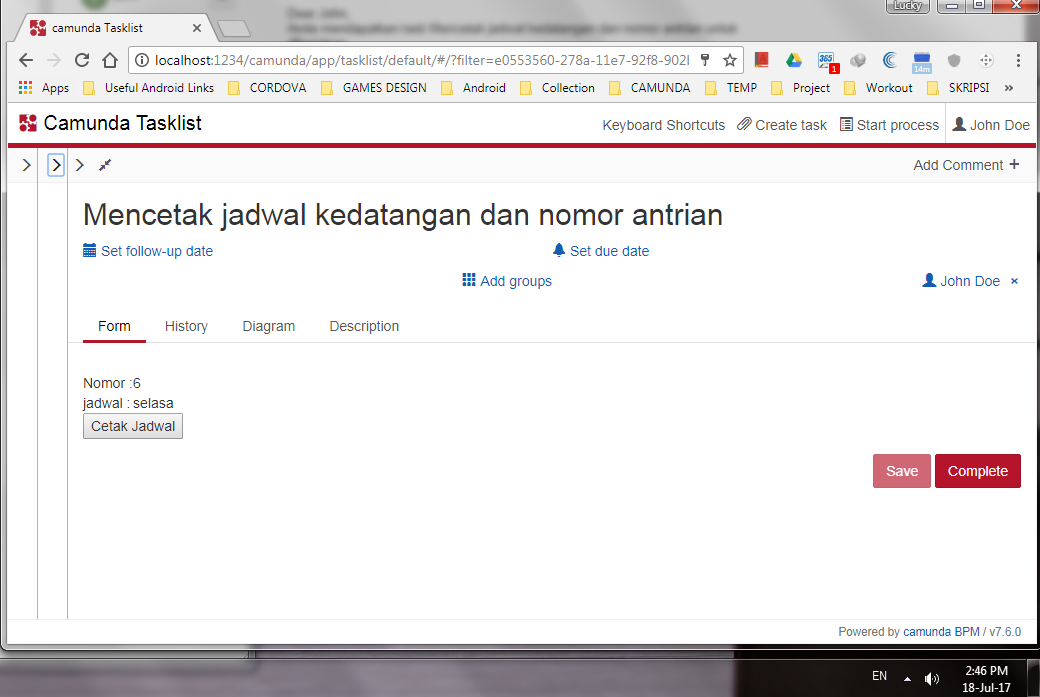
\includegraphics[scale=0.5]{Gambar/Bab-5/kasus2/11}
			\caption{Mencetak Jadwal dan Nomor Antrian} 
			\label{fig:pengujian_kasus2_11}
	\end{figure}
	

	\item Mary, sebagai petugas BPJS menerima email untuk memverifikasi pendaftaran pada pukul 2:46 PM
			\begin{figure}[H]
			\centering
			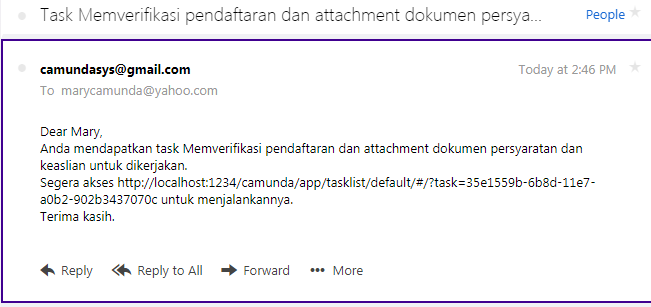
\includegraphics[scale=0.8]{Gambar/Bab-5/kasus2/12}
			\caption{Email Verifikasi Pendaftaran} 
			\label{fig:pengujian_kasus2_12}
	\end{figure}
	

	\item Mary memverifikasi pendaftaran dan semua persyaratan pada pukul 2:47 PM
			\begin{figure}[H]
			\centering
			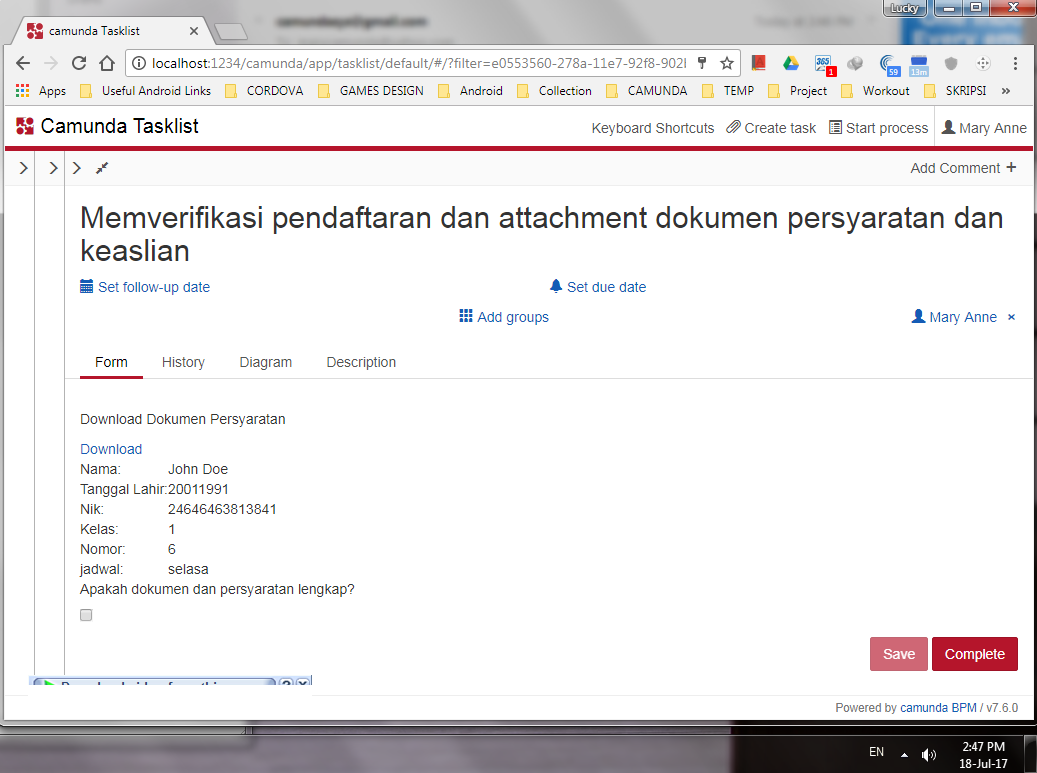
\includegraphics[scale=0.5]{Gambar/Bab-5/kasus2/13}
			\caption{Memverifikasi Pendaftaran dan Semua Persyaratan} 
			\label{fig:pengujian_kasus2_13}
	\end{figure}
	

	\item Mary menerima email untuk mencetak kartu BPJS pada pukul 2:47 PM
			\begin{figure}[H]
			\centering
			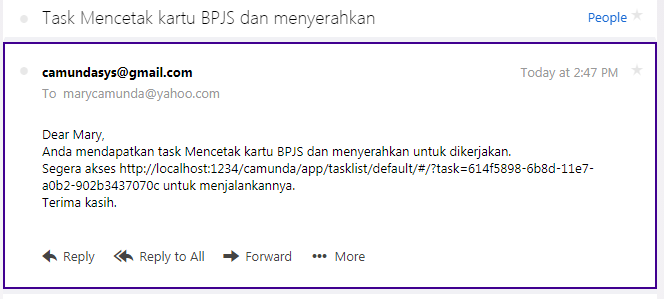
\includegraphics[scale=0.8]{Gambar/Bab-5/kasus2/14}
			\caption{Email Mencetak Kartu BPJS} 
			\label{fig:pengujian_kasus2_14}
	\end{figure}
	

	\item Mary mencetak kartu BPJS pada pukul 2:48 PM
			\begin{figure}[H]
			\centering
			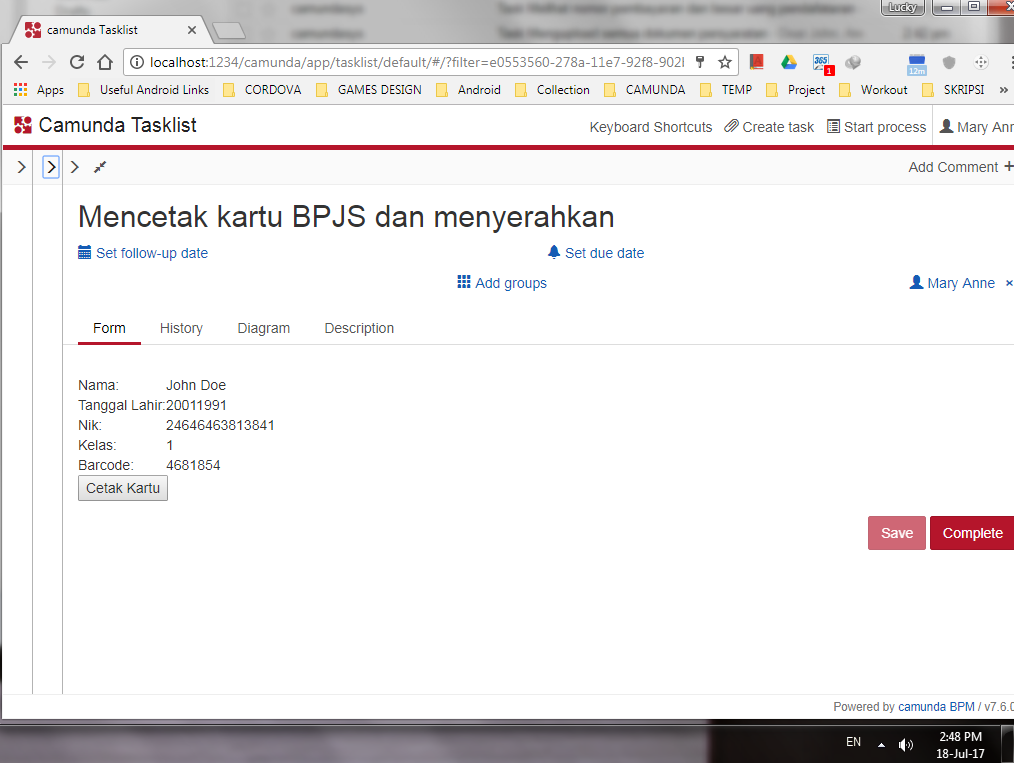
\includegraphics[scale=0.5]{Gambar/Bab-5/kasus2/15}
			\caption{Mencetak Kartu BPJS} 
			\label{fig:pengujian_kasus2_15}
	\end{figure}
\end{enumerate}





		

\section{Analisis Pengujian}
\label{analisispengujian}
Berdasarkan pengujian dua kasus yang telah dilakukan (Pengajuan Proposal dan Pendaftaran BPJS), hasilnya adalah :
\begin{enumerate}
	\item Seluruh \textit{user task} mengirimkan email ke pemilik \textit{task}.
	\item Email langsung dikirim ke pemilik \textit{task} setelah \textit{task} siap dikerjakan. Dapat dilihat dari waktu \textit{task} sebelumnya selesai dan waktu email diterima oleh pemilik \textit{task} yang akan dikerjakan. Misalnya pada kasus Pendaftaran BPJS nomor 13 dan 14, Mary memverifikasi pendaftaran pada pukul 2:47 PM dan menerima email untuk mencetak kartu BPJS (\textit{task} selanjutnya) pada pukul 2:47 PM.
\end{enumerate}
Berdasarkan hasil ini, maka dapat disimpulkan bahwa propagasi email sudah berhasil dilakukan.